%!TEX root = ../thesis.tex
% This paragraph covered a lot of ground, but I was a bit lost since each sentence tried to cover too many different approaches. Is there an implied structure? E.g. first software-static, then software-video, then physical tasks? Id’ have expected some more basic references early on that for example show that people don’t read software documentation and instead look for task-centered learning materials. There’s also a difference between related work that investigates what good instruction formats are, and systems work that introduces new tools to create such formats.

\chapter{Background}

This dissertation proposes computational methods to create interactive tutorials for software applications and physical tasks. To ground our work in existing practices and principles, in this chapter, I define the terminology commonly used by tutorial researchers and online community (Section \ref{background_terms}).
%
I survey research studies and literature about the motivations of people creating, sharing, and consuming tutorials (Section \ref{background_why}) and a common creation process (Section \ref{background_creation}).
%
Finally, I explore the state-of-the-art of technologies that support tutorial authors and learners, including novel interactive format (Section \ref{background_format}) and activity tracking approaches (Section \ref{background_recognition}).

% -------------------------------------------

\section{Instructions: Terminology}
\label{background_terms}

A \keyword{tutorial}, or a \keyword{how-to}, is a representation that transfers domain-specific \keyword{know-how} by describing a set of \keyword{instructions} on how to accomplish a specific \keyword{task}. Instructions have been widely created for various domains, including:

\begin{itemize}
  \itemsep -2pt
  \item Software applications, such as manipulating an image to create a specific blurring effect or creating a pie chart using a spreadsheet application,
  \item Do-It-Yourself (DIY) projects, such as wrapping a gift box or assembling a piece of furniture,
  \item Everyday activities, such as cooking or operating a vacuum machine, and
  \item Sports, such as making a dance move or swing a golf club.
\end{itemize}

Figure~\ref{fig:background_tutorials} shows example activities of the above domains.
\\

% A task-centric tutorial often involves domain-specific \keyword{know-how}, knowledge that is required to perform a task.
%
Often, the instructional content can be structured into a list of steps, which is usually in a linear order, presented as a \keyword{step-by-step} document.
%
In some domains, instructions have been derived into specific formats. For example, cooking recipes contain not only actions but also food ingredients and required amounts.
%
Note that instructions are different from a (software) \keyword{documentation}, \keyword{manual}, or \keyword{user guide} that is a technical document contained non-task-centric details about a particular hardware or software system. To accomplish a task, one may need to identify relevant information from several parts of a manual, instead of following a step-by-step guidance.

Instructions can be shown in different forms. Popular representations include a diagram, written documents that contain text and images, or an instructional video (e.g., screen recording of a software application or a camera recording of a DIY task). Section \ref{background_format} will introduce tutorial formats in details.

\begin{figure*}[t]
  \centering
  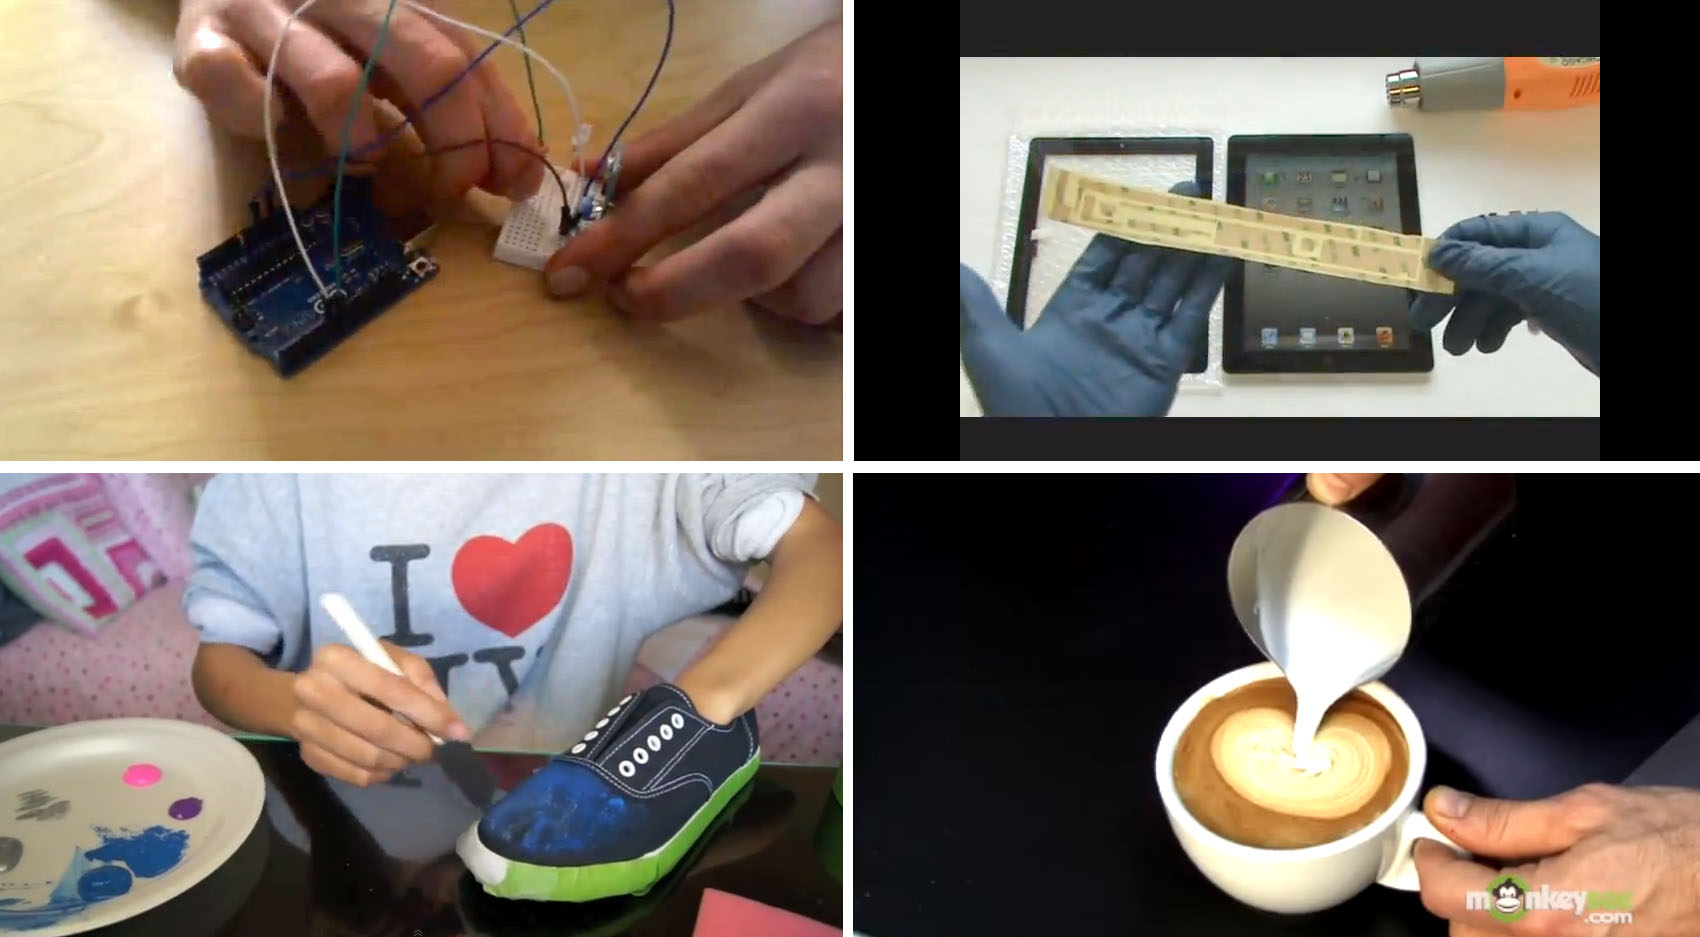
\includegraphics[width=\textwidth]{\background/fig/tutorials}
  \caption{Example activities in tutorial domains: a) image manipulations using a software application, b) a DIY gift-wrapping project, c) cooking as an everyday activity, and d) dancing in sports. \tofix{update the fig}}
  \label{fig:background_tutorials}
\end{figure*}

\subsection{Creating Instructions}
Conventionally, instructions are created by one or more \keyword{authors} who document the process of completing a task and refine the material to a final deliverable.
%
Throughout this dissertation, we call a task completion process as a \keyword{demonstration} or a \keyword{performance}. It can be referred to a \keyword{walkthrough} when using a software application.
%
As the process often involves innovations and creations, authors can also be referred to \keyword{creators} or \keyword{maker}. They are often the \keyword{professionals} or \keyword{experts} in the instructional domains of their work. In tutorial production, however, often they may be \keyword{amateurs} or \keyword{novices} who are not familiar with the tools to refine the documented material.

\subsection{Consuming Instructions}
by viewer, learner, follower
or learning, following -- explain the format in \ref{background_format}

lecturer and online tutoring: involve more feedback collection and response to learners, beyond the scope of this paper

Amateur, expert, professional, novice, hobbyist

interactive tutorials: can be interactively reviewed via software

% -------------------------------------------

\section{Why Instructions?}
\label{background_why}

The research community has been investigating the motivations of both authors and viewers of how-to videos and written tutorials. While one primary motivation is to share expertise, published videos also serve as a way to broadcast skill and as an online portfolio~\cite{Torrey:2007he,Kuznetsov:2010:REA:1868914.1868950}. Authors may derive revenue through advertising or referrals~\cite{Lafreniere:2012tl}. Viewers, on the other hand, typically seek technical explanations, but are also searching for inspiration~\cite{Torrey:2009fc} and looking for validation of existing skills~\cite{Lafreniere:2012tl}.
%
These studies suggest that tutorials have a larger variety of purposes and uses than merely communicating technical content. Recently, guidelines of improving tutorial authorship have been proposed \cite{Wakkary:2015:TAH:2702123.2702550}. Key findings include identifying tools and components and structuring a task into steps with a clear sequence. In our work, we strive to make authoring of instructions more accessible to amateurs while maintaining opportunities for adding individual style through control over editing effects.

Instructables: \cite{Tseng:2014:PVP:2598510.2598540}

% people don’t read software documentation and instead look for task-centered learning materials

% -------------------------------------------

\section{Instruction Creation Process}
\label{background_creation}

\tofix{studies here}

Figure~\ref{fig:background_creation} shows a common workflow of tutorial creation:

\begin{itemize}
  \item \parTitleBold{Planning}:
    Authors make a
  \item \parTitleBold{Capturing}:
    Mutlimedia material is often used to document a process:
    \begin{itemize}
      \itemsep -2pt
      \item Static photographs capture specific moments in a procedure.
      \item Video footages record a computer screencast or a scene of a demonstration.
      \item Audio recordings preserve the sound of activities or author narration.
      \item Other domain-specific content (e.g., code, board layouts, 3D models, and sketches) or resources (e.g., books or URLs to other material) often enrich the instructions.
    \end{itemize}
  \item \parTitleBold{Editing}:
    Once  to make it in a readable or viewable form
  \item \parTitleBold{Reviewing}:
  \item \parTitleBold{Releasing/Sharing}:
    Finally, authors may release the refined content and share the deliverable with others. Common media or platforms include: personal blogs, content sharing sites (e.g., YouTube, Instructables), forums, emails, or private networks.
\end{itemize}

\begin{figure*}[t]
  \centering
  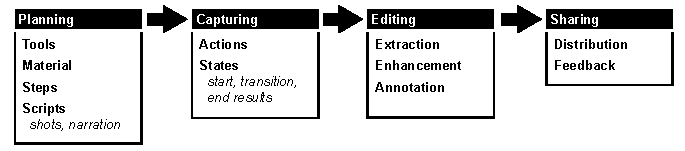
\includegraphics[width=\textwidth]{\background/fig/creation_process}
  \caption{A common workflow of tutorial creation. \tofix{update the fig}}
  \label{fig:background_creation}
\end{figure*}

% -------------------------------------------

\section{Interactive Help and Instruction Formats}
\label{background_format}

There has been a considerable amount of research devoted to tutorial designs that help viewers operate an interactive system. Efforts include visualizing events or embedding instant assistance in software applications and providing real-time feedback on physical tasks.

\subsection{Software Visualization}

In the software application domain, visualizing input and output events has shown to be effective in enhancing instructions. Events can range from low (e.g., mouse actions and movements or keyboard strokes) to high level (e.g., UI component changes). Examples include rendering markers and arrows on screenshot images of a software demo process \cite{Nakamura:2008:ASV:1449715.1449721, Grabler:2009jj}, automatic indexing of instructional software videos \cite{Banovic:2012kd}, and providing visual feedback based on UI operations in real-time \cite{Dixon:2010fb,Dixon:2011:CHP:1978942.1979086}. Work has also aimed to visualize application-centric processes, such as 3D mesh construction \cite{Denning:2011fy} or image manipulation tasks \cite{Grabler:2009jj} as a step-by-step list.

ambient help \cite{Matejka:2011:AH:1978942.1979349}

\subsection{In-Application Support}

Another approach is to provide in-application assistance, often in real-time, in a specific context. Methods include embedding video snippets in application tooltips \cite{Grossman:2010wr}, providing step-by-step wizards \cite{Bergman:2005:DocWizards,Kelleher:2005:STD:1054972.1055047,Fernquist:2011:SRE:2047196.2047245}, automatically navigating video tutorials based on user operations \cite{Pongnumkul:2011ju}, and showing a history of before and after thumbnails and video clips \cite{Grossman:2010jz}. In-app supports can also be dynamically updated within a community based on user contribution \cite{Lafreniere:2013ff,Matejka:2009:CCR:1622176.1622214}.

mobile: EverTutor \cite{Wang:2014:EAC:2556288.2557407}

A Gamified Multiplayer Software Tutorial System \cite{Li:2014:CGM:2556288.2556954}

\subsection{Interactive Tutorial Documents}

Online tutorials
TaggedComments \cite{Bunt:2014:TPI:2556288.2557118}
Steptorials \cite{Lieberman:2014:SML:2557500.2557543} -- high-functionality (hi-fun) application

\subsection{Instructions for Physical Tasks}

Beyond software applications to the real world where activity and object recognition is difficult, researchers have investigated tools for supporting physical tasks. Workflows can be automatically generated for furniture \cite{agrawala2003designing} or block assembly tasks \cite{Gupta:2012ku}; the latter was shown to be trackable for real-time guidance.
%
Information can also be overlaid on top of the work area using augmented reality, usually through a head-mounted display. Such systems can provide visual highlights for machine maintenance \cite{Henderson:2011ff}, or interactive remote tutoring for repair tasks~\cite{Gurevich:2012ko}. Another method is to overlay guidance on an augmented mirror for tasks such as dance movements \cite{Anderson:2013:YEM:2501988.2502045}.

table for physical tasks \cite{Knibbe:2015:SMI:2817721.2817741}

spin: photo turntable \cite{Tseng:2015:SPT:2771839.2771869}
documentation \cite{Tseng:2016:makeology}

These projects show how effective instructional representations can assist learners in learning or executing tasks. Our goal is to further study new formats that incorporate advantages of several formats of multimedia, including images, text, and videos, and in turn enhancing the learning experience for a variety of tasks.

% add some Tiffany Tseng's work
% http://web.mit.edu/ttseng/www/academics/index.html

% -------------------------------------------

\section{Activity Tracking for Creating and Following Instructions}
\label{background_recognition}

* define ``automatic''
% Note: MixT tutorials are automatically rendered from manual demonstration, not automatically generated.

To provide real-time assistance, it is important to recognize the user activities during a task performance. Several domains have been widely studied, including software operations, scene recognition, and object tracking in a physical world.
%
Researchers have shown that workflows and content of desktop applications can be captured automatically using computer vision \cite{Yeh:2009dh,Chang:2011vd} and application logs \cite{Grossman:2010jz,Grabler:2009jj,Pongnumkul:2011ju}.
%
However, tracking user behavior in the physical world, rather than in software, remains a challenge. Computer vision techniques can track specific targets, including hands \cite{Ranjan:2008}, user movements \cite{Wilson:2012fb}, fast-moving objects (e.g., a Ping-Pong ball) \cite{Okumura:2011tr}, or regions in pre-defined spaces \cite{Ranjan:2007}.

These methods usually require an expert defining heuristics of space regions or movement classifications ahead of time for the tracking program.
%
On the contrary, we propose a new approach that does not have these issues, gives users flexibility in a home environment, and provides interactive control. If activity recognition is not possible, we include users in the loop to annotate high-level information in order to create high-quality results.
%
Emerging work has provided insights toward this vision using consumer devices such as a Kinect sensor \cite{Anderson:2013:YEM:2501988.2502045,Gupta:2012ku} to provide dynamic instructions, which shares a similar goal with ours.

% -------------------------------------------

% \section{Video Capture, Annotation and Editing}
% \subsubTitleI{Capture} Several research and commercial systems guide users at capture time to yield higher-quality videos. Such systems often employ templates to help users capture sequences of distinct shots (e.g., Snapguide\footnote{http://snapguide.com/}) or suggest framing of the subject or camera view as in NudgeCam~\cite{Carter:2010}. Computer vision algorithms, like face tracking, can be used to offer real-time feedback during such directed actions~\cite{Davis:2003cu,Heer:2004ba,Carter:2010}. Instead of relying on templates, shot suggestions can also be bootstrapped through user dialogs~\cite{Adams:2005}.

% \subsubTitleI{Annotation} Researchers have investigated how to provide interactions that enable efficient, fluid annotation of video data, from the early EVA system~\cite{Mackay:1989} to more recent interfaces like VideoTater that leverage pen input~\cite{Diakopoulos:2006vt}. We do not claim a contribution in the interaction techniques of our annotation interface and take inspiration from such prior work.

% \subsubTitleI{Editing} Frame-based editing of video is very time-intensive, as it forces users to operate at a very low level of detail. Editors can leverage metadata, such as transcripts~\cite{Berthouzoz:2012,Pavel:2014:VDB:2642918.2647400} and shot boundaries~\cite{Casares:2002dx}, to give users higher-level editing operations at the shot level rather than the frame level.
%In specific video domains like interview videos, transcripts can help users place cuts and transitions~\cite{Berthouzoz:2012}.
Computer vision techniques can automate certain effects, such as creating cinemagraphs~\cite{Bai:2012, Joshi:2012}, automatically-edited lecture videos~\cite{Heck:2007}, zoomable tapestries~\cite{Barnes:2010} and synopses~\cite{Pritch:2009vl}, or stabilizing shaky amateur videos~\cite{Liu:2011}. When analyzing video is a matter of subjective taste, identifying salient frames can also be outsourced to crowd workers~\cite{Bernstein:2011uj}.

In contrast to these systems, we do not require the author to manipulate the camera or system during capture. Many leisure activities, such as home repair or cooking, require use of both hands or involve getting one's hands dirty, so camera manipulation is not possible. We use vision techniques for automatic recording and editing. It differs from previous approaches in its focus on particular application domains -- software and physical demonstrations. By focusing on specific domains, we can make assumptions about the structure of the input and output video, such as the fact that there is a linear set of steps or movements, and offer user interfaces and algorithms that make it easier to create high quality instructions.
